% Options for packages loaded elsewhere
\PassOptionsToPackage{unicode}{hyperref}
\PassOptionsToPackage{hyphens}{url}
%
\documentclass[
]{article}
\usepackage{lmodern}
\usepackage{amssymb,amsmath}
\usepackage{ifxetex,ifluatex}
\ifnum 0\ifxetex 1\fi\ifluatex 1\fi=0 % if pdftex
  \usepackage[T1]{fontenc}
  \usepackage[utf8]{inputenc}
  \usepackage{textcomp} % provide euro and other symbols
\else % if luatex or xetex
  \usepackage{unicode-math}
  \defaultfontfeatures{Scale=MatchLowercase}
  \defaultfontfeatures[\rmfamily]{Ligatures=TeX,Scale=1}
\fi
% Use upquote if available, for straight quotes in verbatim environments
\IfFileExists{upquote.sty}{\usepackage{upquote}}{}
\IfFileExists{microtype.sty}{% use microtype if available
  \usepackage[]{microtype}
  \UseMicrotypeSet[protrusion]{basicmath} % disable protrusion for tt fonts
}{}
\makeatletter
\@ifundefined{KOMAClassName}{% if non-KOMA class
  \IfFileExists{parskip.sty}{%
    \usepackage{parskip}
  }{% else
    \setlength{\parindent}{0pt}
    \setlength{\parskip}{6pt plus 2pt minus 1pt}}
}{% if KOMA class
  \KOMAoptions{parskip=half}}
\makeatother
\usepackage{xcolor}
\IfFileExists{xurl.sty}{\usepackage{xurl}}{} % add URL line breaks if available
\IfFileExists{bookmark.sty}{\usepackage{bookmark}}{\usepackage{hyperref}}
\hypersetup{
  pdftitle={Psy/Educ 6600: Unit 5 Homework},
  pdfauthor={Your Name},
  hidelinks,
  pdfcreator={LaTeX via pandoc}}
\urlstyle{same} % disable monospaced font for URLs
\usepackage[margin=1in]{geometry}
\usepackage{color}
\usepackage{fancyvrb}
\newcommand{\VerbBar}{|}
\newcommand{\VERB}{\Verb[commandchars=\\\{\}]}
\DefineVerbatimEnvironment{Highlighting}{Verbatim}{commandchars=\\\{\}}
% Add ',fontsize=\small' for more characters per line
\usepackage{framed}
\definecolor{shadecolor}{RGB}{248,248,248}
\newenvironment{Shaded}{\begin{snugshade}}{\end{snugshade}}
\newcommand{\AlertTok}[1]{\textcolor[rgb]{0.94,0.16,0.16}{#1}}
\newcommand{\AnnotationTok}[1]{\textcolor[rgb]{0.56,0.35,0.01}{\textbf{\textit{#1}}}}
\newcommand{\AttributeTok}[1]{\textcolor[rgb]{0.77,0.63,0.00}{#1}}
\newcommand{\BaseNTok}[1]{\textcolor[rgb]{0.00,0.00,0.81}{#1}}
\newcommand{\BuiltInTok}[1]{#1}
\newcommand{\CharTok}[1]{\textcolor[rgb]{0.31,0.60,0.02}{#1}}
\newcommand{\CommentTok}[1]{\textcolor[rgb]{0.56,0.35,0.01}{\textit{#1}}}
\newcommand{\CommentVarTok}[1]{\textcolor[rgb]{0.56,0.35,0.01}{\textbf{\textit{#1}}}}
\newcommand{\ConstantTok}[1]{\textcolor[rgb]{0.00,0.00,0.00}{#1}}
\newcommand{\ControlFlowTok}[1]{\textcolor[rgb]{0.13,0.29,0.53}{\textbf{#1}}}
\newcommand{\DataTypeTok}[1]{\textcolor[rgb]{0.13,0.29,0.53}{#1}}
\newcommand{\DecValTok}[1]{\textcolor[rgb]{0.00,0.00,0.81}{#1}}
\newcommand{\DocumentationTok}[1]{\textcolor[rgb]{0.56,0.35,0.01}{\textbf{\textit{#1}}}}
\newcommand{\ErrorTok}[1]{\textcolor[rgb]{0.64,0.00,0.00}{\textbf{#1}}}
\newcommand{\ExtensionTok}[1]{#1}
\newcommand{\FloatTok}[1]{\textcolor[rgb]{0.00,0.00,0.81}{#1}}
\newcommand{\FunctionTok}[1]{\textcolor[rgb]{0.00,0.00,0.00}{#1}}
\newcommand{\ImportTok}[1]{#1}
\newcommand{\InformationTok}[1]{\textcolor[rgb]{0.56,0.35,0.01}{\textbf{\textit{#1}}}}
\newcommand{\KeywordTok}[1]{\textcolor[rgb]{0.13,0.29,0.53}{\textbf{#1}}}
\newcommand{\NormalTok}[1]{#1}
\newcommand{\OperatorTok}[1]{\textcolor[rgb]{0.81,0.36,0.00}{\textbf{#1}}}
\newcommand{\OtherTok}[1]{\textcolor[rgb]{0.56,0.35,0.01}{#1}}
\newcommand{\PreprocessorTok}[1]{\textcolor[rgb]{0.56,0.35,0.01}{\textit{#1}}}
\newcommand{\RegionMarkerTok}[1]{#1}
\newcommand{\SpecialCharTok}[1]{\textcolor[rgb]{0.00,0.00,0.00}{#1}}
\newcommand{\SpecialStringTok}[1]{\textcolor[rgb]{0.31,0.60,0.02}{#1}}
\newcommand{\StringTok}[1]{\textcolor[rgb]{0.31,0.60,0.02}{#1}}
\newcommand{\VariableTok}[1]{\textcolor[rgb]{0.00,0.00,0.00}{#1}}
\newcommand{\VerbatimStringTok}[1]{\textcolor[rgb]{0.31,0.60,0.02}{#1}}
\newcommand{\WarningTok}[1]{\textcolor[rgb]{0.56,0.35,0.01}{\textbf{\textit{#1}}}}
\usepackage{longtable,booktabs}
% Correct order of tables after \paragraph or \subparagraph
\usepackage{etoolbox}
\makeatletter
\patchcmd\longtable{\par}{\if@noskipsec\mbox{}\fi\par}{}{}
\makeatother
% Allow footnotes in longtable head/foot
\IfFileExists{footnotehyper.sty}{\usepackage{footnotehyper}}{\usepackage{footnote}}
\makesavenoteenv{longtable}
\usepackage{graphicx,grffile}
\makeatletter
\def\maxwidth{\ifdim\Gin@nat@width>\linewidth\linewidth\else\Gin@nat@width\fi}
\def\maxheight{\ifdim\Gin@nat@height>\textheight\textheight\else\Gin@nat@height\fi}
\makeatother
% Scale images if necessary, so that they will not overflow the page
% margins by default, and it is still possible to overwrite the defaults
% using explicit options in \includegraphics[width, height, ...]{}
\setkeys{Gin}{width=\maxwidth,height=\maxheight,keepaspectratio}
% Set default figure placement to htbp
\makeatletter
\def\fps@figure{htbp}
\makeatother
\usepackage[normalem]{ulem}
% Avoid problems with \sout in headers with hyperref
\pdfstringdefDisableCommands{\renewcommand{\sout}{}}
\setlength{\emergencystretch}{3em} % prevent overfull lines
\providecommand{\tightlist}{%
  \setlength{\itemsep}{0pt}\setlength{\parskip}{0pt}}
\setcounter{secnumdepth}{-\maxdimen} % remove section numbering

\title{Psy/Educ 6600: Unit 5 Homework}
\usepackage{etoolbox}
\makeatletter
\providecommand{\subtitle}[1]{% add subtitle to \maketitle
  \apptocmd{\@title}{\par {\large #1 \par}}{}{}
}
\makeatother
\subtitle{ANOVA - With Repeated Measures}
\author{Your Name}
\date{Spring 2020}

\begin{document}
\maketitle

{
\setcounter{tocdepth}{3}
\tableofcontents
}
\clearpage

\hypertarget{preparation}{%
\section{PREPARATION}\label{preparation}}

\hypertarget{packages}{%
\subsection{Packages}\label{packages}}

Make sure the packages are \textbf{installed} \emph{(Package tab)}

\begin{Shaded}
\begin{Highlighting}[]
\KeywordTok{library}\NormalTok{(magrittr)}
\KeywordTok{library}\NormalTok{(tidyverse)    }\CommentTok{# Loads several very helpful 'tidy' packages}
\KeywordTok{library}\NormalTok{(readxl)       }\CommentTok{# Read in Excel datasets}
\KeywordTok{library}\NormalTok{(furniture)    }\CommentTok{# Nice tables (by our own Tyson Barrett)}
\KeywordTok{library}\NormalTok{(afex)         }\CommentTok{# Analysis of Factorial Experiments}
\KeywordTok{library}\NormalTok{(emmeans)      }\CommentTok{# Estimated marginal means (Least-squares means)}
\KeywordTok{library}\NormalTok{(lsmeans)      }\CommentTok{# Least-Squares Means}
\KeywordTok{library}\NormalTok{(multcomp)     }\CommentTok{# Simultaneous Inference in General Parametric Models }
\KeywordTok{library}\NormalTok{(pander)       }\CommentTok{# Formats tables }
\end{Highlighting}
\end{Shaded}

\clearpage

\hypertarget{section-b}{%
\section{SECTION B}\label{section-b}}

\hypertarget{datasets}{%
\subsection{Datasets}\label{datasets}}

\begin{Shaded}
\begin{Highlighting}[]
\NormalTok{memory_wide <-}\StringTok{ }\KeywordTok{data.frame}\NormalTok{(}\DataTypeTok{id =} \DecValTok{1}\OperatorTok{:}\DecValTok{6}\NormalTok{,}
                          \DataTypeTok{digit  =} \KeywordTok{c}\NormalTok{(}\DecValTok{6}\NormalTok{, }\DecValTok{8}\NormalTok{, }\DecValTok{7}\NormalTok{, }\DecValTok{8}\NormalTok{, }\DecValTok{6}\NormalTok{, }\DecValTok{7}\NormalTok{),}
                          \DataTypeTok{letter =} \KeywordTok{c}\NormalTok{(}\DecValTok{5}\NormalTok{, }\DecValTok{7}\NormalTok{, }\DecValTok{7}\NormalTok{, }\DecValTok{5}\NormalTok{, }\DecValTok{4}\NormalTok{, }\DecValTok{6}\NormalTok{),}
                          \DataTypeTok{mixed  =} \KeywordTok{c}\NormalTok{(}\DecValTok{6}\NormalTok{, }\DecValTok{5}\NormalTok{, }\DecValTok{4}\NormalTok{, }\DecValTok{8}\NormalTok{, }\DecValTok{7}\NormalTok{, }\DecValTok{5}\NormalTok{)) }\OperatorTok\StringTok{ }
\StringTok{  }\NormalTok{dplyr}\OperatorTok{::}\KeywordTok{mutate}\NormalTok{(}\DataTypeTok{id =} \KeywordTok{factor}\NormalTok{(id))}


\NormalTok{caffiene_wide <-}\StringTok{ }\KeywordTok{data.frame}\NormalTok{(}\DataTypeTok{block  =} \DecValTok{1}\OperatorTok{:}\DecValTok{6}\NormalTok{,}
                           \DataTypeTok{mg_0   =} \KeywordTok{c}\NormalTok{(}\DecValTok{25}\NormalTok{, }\DecValTok{19}\NormalTok{, }\DecValTok{22}\NormalTok{, }\DecValTok{15}\NormalTok{, }\DecValTok{16}\NormalTok{, }\DecValTok{20}\NormalTok{),}
                           \DataTypeTok{mg_100 =} \KeywordTok{c}\NormalTok{(}\DecValTok{16}\NormalTok{, }\DecValTok{15}\NormalTok{, }\DecValTok{19}\NormalTok{, }\DecValTok{11}\NormalTok{, }\DecValTok{14}\NormalTok{, }\DecValTok{23}\NormalTok{),}
                           \DataTypeTok{mg_200 =} \KeywordTok{c}\NormalTok{( }\DecValTok{6}\NormalTok{, }\DecValTok{14}\NormalTok{,  }\DecValTok{9}\NormalTok{,  }\DecValTok{5}\NormalTok{,  }\DecValTok{9}\NormalTok{, }\DecValTok{11}\NormalTok{),}
                           \DataTypeTok{mg_300 =} \KeywordTok{c}\NormalTok{( }\DecValTok{8}\NormalTok{, }\DecValTok{18}\NormalTok{,  }\DecValTok{9}\NormalTok{, }\DecValTok{10}\NormalTok{, }\DecValTok{12}\NormalTok{, }\DecValTok{13}\NormalTok{)) }\OperatorTok\StringTok{ }
\StringTok{  }\NormalTok{dplyr}\OperatorTok{::}\KeywordTok{mutate}\NormalTok{(}\DataTypeTok{block =} \KeywordTok{factor}\NormalTok{(block))}


\NormalTok{audience_wide <-}\StringTok{ }\KeywordTok{data.frame}\NormalTok{(}\DataTypeTok{id     =} \DecValTok{1}\OperatorTok{:}\DecValTok{12}\NormalTok{,}
                            \DataTypeTok{one    =} \KeywordTok{c}\NormalTok{(}\DecValTok{131}\NormalTok{, }\DecValTok{109}\NormalTok{, }\DecValTok{115}\NormalTok{, }\DecValTok{110}\NormalTok{, }\DecValTok{107}\NormalTok{, }\DecValTok{111}\NormalTok{, }
                                       \DecValTok{100}\NormalTok{, }\DecValTok{115}\NormalTok{, }\DecValTok{130}\NormalTok{, }\DecValTok{118}\NormalTok{, }\DecValTok{125}\NormalTok{, }\DecValTok{135}\NormalTok{),}
                            \DataTypeTok{twenty =} \KeywordTok{c}\NormalTok{(}\DecValTok{130}\NormalTok{, }\DecValTok{124}\NormalTok{, }\DecValTok{110}\NormalTok{, }\DecValTok{108}\NormalTok{, }\DecValTok{115}\NormalTok{, }\DecValTok{117}\NormalTok{, }
                                       \DecValTok{102}\NormalTok{, }\DecValTok{120}\NormalTok{, }\DecValTok{119}\NormalTok{, }\DecValTok{122}\NormalTok{, }\DecValTok{118}\NormalTok{, }\DecValTok{130}\NormalTok{),}
                            \DataTypeTok{large  =} \KeywordTok{c}\NormalTok{(}\DecValTok{135}\NormalTok{, }\DecValTok{126}\NormalTok{, }\DecValTok{108}\NormalTok{, }\DecValTok{122}\NormalTok{, }\DecValTok{111}\NormalTok{, }\DecValTok{121}\NormalTok{, }
                                       \DecValTok{107}\NormalTok{, }\DecValTok{132}\NormalTok{, }\DecValTok{128}\NormalTok{, }\DecValTok{130}\NormalTok{, }\DecValTok{133}\NormalTok{, }\DecValTok{135}\NormalTok{))}\OperatorTok\StringTok{ }
\StringTok{  }\NormalTok{dplyr}\OperatorTok{::}\KeywordTok{mutate}\NormalTok{(}\DataTypeTok{id =} \KeywordTok{factor}\NormalTok{(id))}

\NormalTok{textbook_wide <-}\StringTok{ }\KeywordTok{data.frame}\NormalTok{(}\DataTypeTok{block =} \DecValTok{1}\OperatorTok{:}\DecValTok{9}\NormalTok{,}
                            \DataTypeTok{A =} \KeywordTok{c}\NormalTok{(}\DecValTok{17}\NormalTok{,  }\DecValTok{8}\NormalTok{,  }\DecValTok{6}\NormalTok{, }\DecValTok{12}\NormalTok{, }\DecValTok{19}\NormalTok{, }\DecValTok{14}\NormalTok{, }\DecValTok{10}\NormalTok{,  }\DecValTok{7}\NormalTok{, }\DecValTok{12}\NormalTok{),}
                            \DataTypeTok{B =} \KeywordTok{c}\NormalTok{(}\DecValTok{15}\NormalTok{,  }\DecValTok{6}\NormalTok{,  }\DecValTok{5}\NormalTok{, }\DecValTok{10}\NormalTok{, }\DecValTok{20}\NormalTok{, }\DecValTok{13}\NormalTok{,  }\DecValTok{7}\NormalTok{,  }\DecValTok{7}\NormalTok{, }\DecValTok{11}\NormalTok{),}
                            \DataTypeTok{C =} \KeywordTok{c}\NormalTok{(}\DecValTok{20}\NormalTok{, }\DecValTok{11}\NormalTok{, }\DecValTok{10}\NormalTok{, }\DecValTok{14}\NormalTok{, }\DecValTok{20}\NormalTok{, }\DecValTok{15}\NormalTok{, }\DecValTok{14}\NormalTok{, }\DecValTok{11}\NormalTok{, }\DecValTok{15}\NormalTok{),}
                            \DataTypeTok{D =} \KeywordTok{c}\NormalTok{(}\DecValTok{18}\NormalTok{,  }\DecValTok{7}\NormalTok{,  }\DecValTok{6}\NormalTok{, }\DecValTok{13}\NormalTok{, }\DecValTok{18}\NormalTok{, }\DecValTok{15}\NormalTok{, }\DecValTok{10}\NormalTok{,  }\DecValTok{6}\NormalTok{, }\DecValTok{13}\NormalTok{))}\OperatorTok\StringTok{ }
\StringTok{  }\NormalTok{dplyr}\OperatorTok{::}\KeywordTok{mutate}\NormalTok{(}\DataTypeTok{block =} \KeywordTok{factor}\NormalTok{(block))}
\end{Highlighting}
\end{Shaded}

\clearpage

\hypertarget{memory_wide}{%
\subsection{\texorpdfstring{\texttt{memory\_wide}}{memory\_wide}}\label{memory_wide}}

\begin{Shaded}
\begin{Highlighting}[]
\NormalTok{memory_wide}
\end{Highlighting}
\end{Shaded}

\begin{verbatim}
  id digit letter mixed
1  1     6      5     6
2  2     8      7     5
3  3     7      7     4
4  4     8      5     8
5  5     6      4     7
6  6     7      6     5
\end{verbatim}

\hypertarget{restructure-from-wide-to-long-format}{%
\subsubsection{Restructure from wide to long
format}\label{restructure-from-wide-to-long-format}}

\begin{Shaded}
\begin{Highlighting}[]
\NormalTok{memory_long <-}\StringTok{ }\NormalTok{memory_wide }\OperatorTok\StringTok{ }
\StringTok{  }\NormalTok{tidyr}\OperatorTok{::}\KeywordTok{pivot_longer}\NormalTok{(}\DataTypeTok{cols =} \KeywordTok{c}\NormalTok{(digit, letter, mixed),}
                      \DataTypeTok{names_to =} \StringTok{"stimuli"}\NormalTok{,}
                      \DataTypeTok{names_ptypes =} \KeywordTok{list}\NormalTok{(}\DataTypeTok{stimuli =} \KeywordTok{factor}\NormalTok{()),}
                      \DataTypeTok{values_to =} \StringTok{"recall"}\NormalTok{)}

\NormalTok{psych}\OperatorTok{::}\KeywordTok{headTail}\NormalTok{(memory_long)}
\end{Highlighting}
\end{Shaded}

\begin{verbatim}
    id stimuli recall
1    1   digit      6
2    1  letter      5
3    1   mixed      6
4    2   digit      8
5 <NA>    <NA>    ...
6    5   mixed      7
7    6   digit      7
8    6  letter      6
9    6   mixed      5
\end{verbatim}

\hypertarget{person-profile-plot}{%
\subsubsection{Person-Profile Plot}\label{person-profile-plot}}

\begin{Shaded}
\begin{Highlighting}[]
\NormalTok{memory_long }\OperatorTok\StringTok{ }
\StringTok{  }\KeywordTok{ggplot}\NormalTok{(}\KeywordTok{aes}\NormalTok{(}\DataTypeTok{x =}\NormalTok{ stimuli,}
             \DataTypeTok{y =}\NormalTok{ recall,}
             \DataTypeTok{group =}\NormalTok{ id,}
             \DataTypeTok{linetype =}\NormalTok{ id)) }\OperatorTok{+}
\StringTok{  }\KeywordTok{geom_point}\NormalTok{()}\OperatorTok{+}
\StringTok{  }\KeywordTok{geom_line}\NormalTok{()}
\end{Highlighting}
\end{Shaded}

\begin{center}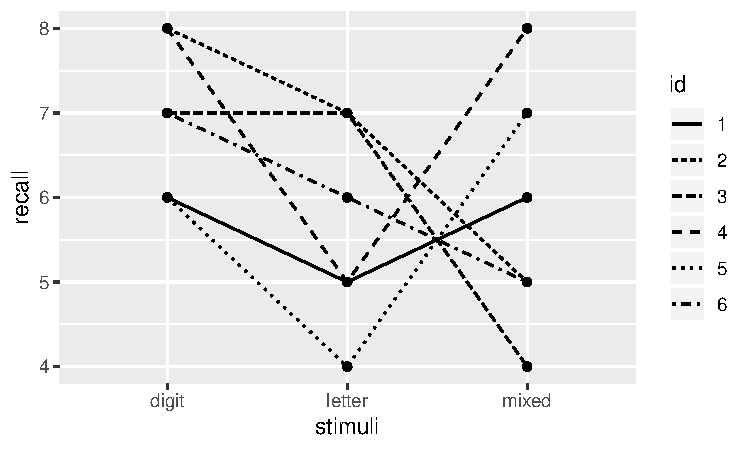
\includegraphics{Chapter-15-Assignment-R-Skeleton--2020spring_files/figure-latex/unnamed-chunk-3-1} \end{center}

\clearpage

\hypertarget{caffiene_wide}{%
\subsection{\texorpdfstring{\texttt{caffiene\_wide}}{caffiene\_wide}}\label{caffiene_wide}}

\begin{Shaded}
\begin{Highlighting}[]
\NormalTok{caffiene_wide}
\end{Highlighting}
\end{Shaded}

\begin{verbatim}
  block mg_0 mg_100 mg_200 mg_300
1     1   25     16      6      8
2     2   19     15     14     18
3     3   22     19      9      9
4     4   15     11      5     10
5     5   16     14      9     12
6     6   20     23     11     13
\end{verbatim}

\hypertarget{restructure-from-wide-to-long-format-1}{%
\subsubsection{Restructure from wide to long
format}\label{restructure-from-wide-to-long-format-1}}

\begin{Shaded}
\begin{Highlighting}[]
\NormalTok{caffiene_long <-}\StringTok{ }\NormalTok{caffiene_wide }\OperatorTok\StringTok{ }
\StringTok{  }\NormalTok{tidyr}\OperatorTok{::}\KeywordTok{pivot_longer}\NormalTok{(}\DataTypeTok{cols =} \KeywordTok{c}\NormalTok{(mg_}\DecValTok{0}\NormalTok{, mg_}\DecValTok{100}\NormalTok{, mg_}\DecValTok{200}\NormalTok{, mg_}\DecValTok{300}\NormalTok{),}
                      \DataTypeTok{names_to =} \StringTok{"dose"}\NormalTok{,}
                      \DataTypeTok{names_prefix =} \StringTok{"mg_"}\NormalTok{,}
                      \DataTypeTok{names_ptypes =} \KeywordTok{list}\NormalTok{(}\DataTypeTok{dose =} \KeywordTok{factor}\NormalTok{()),}
                      \DataTypeTok{values_to =} \StringTok{"errors"}\NormalTok{)}

\NormalTok{psych}\OperatorTok{::}\KeywordTok{headTail}\NormalTok{(caffiene_long)}
\end{Highlighting}
\end{Shaded}

\begin{verbatim}
  block dose errors
1     1    0     25
2     1  100     16
3     1  200      6
4     1  300      8
5  <NA> <NA>    ...
6     6    0     20
7     6  100     23
8     6  200     11
9     6  300     13
\end{verbatim}

\hypertarget{person-profile-plot-1}{%
\subsubsection{Person-Profile Plot}\label{person-profile-plot-1}}

\begin{Shaded}
\begin{Highlighting}[]
\NormalTok{caffiene_long }\OperatorTok\StringTok{ }
\StringTok{  }\KeywordTok{ggplot}\NormalTok{(}\KeywordTok{aes}\NormalTok{(}\DataTypeTok{x =}\NormalTok{ dose,}
             \DataTypeTok{y =}\NormalTok{ errors,}
             \DataTypeTok{group =}\NormalTok{ block,}
             \DataTypeTok{linetype =}\NormalTok{ block)) }\OperatorTok{+}
\StringTok{  }\KeywordTok{geom_point}\NormalTok{()}\OperatorTok{+}
\StringTok{  }\KeywordTok{geom_line}\NormalTok{()}
\end{Highlighting}
\end{Shaded}

\begin{center}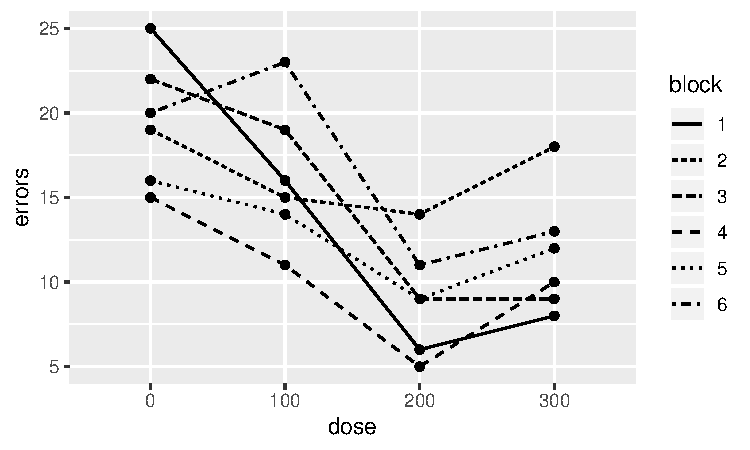
\includegraphics{Chapter-15-Assignment-R-Skeleton--2020spring_files/figure-latex/unnamed-chunk-6-1} \end{center}

\clearpage

\hypertarget{audience_wide---repeated-measures-design-effect-of-audience-size-on-blood-pressure}{%
\subsection{\texorpdfstring{\texttt{audience\_wide} - Repeated Measures
Design: Effect of Audience Size on Blood
Pressure}{audience\_wide - Repeated Measures Design: Effect of Audience Size on Blood Pressure}}\label{audience_wide---repeated-measures-design-effect-of-audience-size-on-blood-pressure}}

\textbf{TEXTBOOK QUESTION:} \emph{A psychophysiologist wishes to explore
the effects of public speaking on the systolic blood pressure of young
adults. Three conditions are tested. The subject must vividly imagine
delivering a speech to one person, to a small class of 20 persons, or to
a large audience consisting of hundreds of fellow students. Each subject
has his or her systolic blood pressure measured (mmHg) under all three
conditions. Two subjects are randomly assigned to each of the six
possible treatment orders. The data appear in the following table:}

\begin{verbatim}
   id one twenty large
1   1 131    130   135
2   2 109    124   126
3   3 115    110   108
4   4 110    108   122
5   5 107    115   111
6   6 111    117   121
7   7 100    102   107
8   8 115    120   132
9   9 130    119   128
10 10 118    122   130
11 11 125    118   133
12 12 135    130   135
\end{verbatim}

\hypertarget{restructure-from-wide-to-long-format-2}{%
\subsubsection{Restructure from wide to long
format}\label{restructure-from-wide-to-long-format-2}}

\begin{verbatim}
    id audience blood_pressure
1    1      one            131
2    1   twenty            130
3    1    large            135
4    2      one            109
5 <NA>     <NA>            ...
6   11    large            133
7   12      one            135
8   12   twenty            130
9   12    large            135
\end{verbatim}

\clearpage

\hypertarget{summary-statistics}{%
\subsubsection{Summary Statistics}\label{summary-statistics}}

\begin{longtable}[]{@{}llll@{}}
\toprule
& one & twenty & large\tabularnewline
\midrule
\endhead
& n = 12 & n = 12 & n = 12\tabularnewline
blood\_pressure & & &\tabularnewline
& 117.2 (10.9) & 117.9 (8.4) & 124.0 (10.3)\tabularnewline
\bottomrule
\end{longtable}

\hypertarget{person-profile-plot-2}{%
\subsubsection{Person-Profile Plot}\label{person-profile-plot-2}}

\begin{center}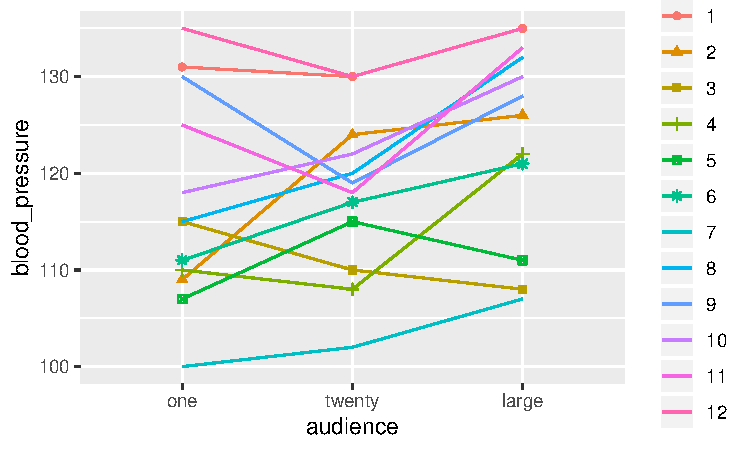
\includegraphics{Chapter-15-Assignment-R-Skeleton--2020spring_files/figure-latex/unnamed-chunk-11-1} \end{center}

\hypertarget{means-plot}{%
\subsubsection{Means Plot}\label{means-plot}}

\begin{center}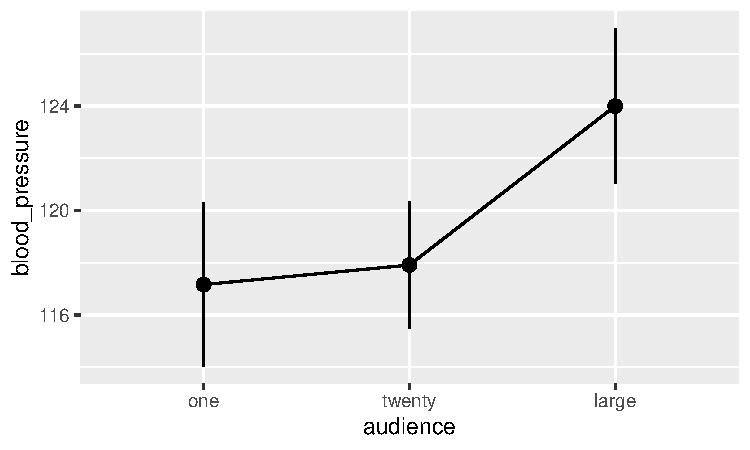
\includegraphics{Chapter-15-Assignment-R-Skeleton--2020spring_files/figure-latex/unnamed-chunk-12-1} \end{center}

\clearpage

\hypertarget{b-3abc-rm-anova-no-sphericity-correction-but-both-effect-sizes}{%
\subsubsection{15B-3a/b/c RM ANOVA: no sphericity correction, but both
effect
sizes}\label{b-3abc-rm-anova-no-sphericity-correction-but-both-effect-sizes}}

\textbf{TEXTBOOK QUESTION:} \emph{(a) Perform an RM ANOVA on the blood
pressure data and write the results in words, as they would appear in a
journal article. Does the size of the audience have a significant effect
on blood pressure at the .05 level? \sout{(Hint : Subtract 100 from
every entry in the preceding table before computing any of the SS's.
This will make your work easier without changing any of the SS
components or F ratios.)} (b) What might you do to minimize the
possibility of carryover effects?}

\textbf{DIRECTIONS:} Perform a Repeated Measures ANOVA for blood
pressure under the three condiditons to determine if the size of the
imagine audience has an effect. Request no correction for violations of
sphericity (\texttt{correction\ =\ "none"}) and both effect sizes
(\texttt{es\ =\ c("ges",\ "pes"}). Save this model as a name
\texttt{fit\_audience} and run the name (without \texttt{\$Anova}) to
see the brief output.

\begin{Shaded}
\begin{Highlighting}[]
\CommentTok{# RM ANOVA: no correction for lack of sphericity  <-- NAME AND SAVE}
\end{Highlighting}
\end{Shaded}

\clearpage

\hypertarget{b-3c-rm-anova-display-all-sums-of-squares-components}{%
\subsubsection{15B-3c RM ANOVA: display all Sums-of-Squares
components}\label{b-3c-rm-anova-display-all-sums-of-squares-components}}

\textbf{TEXTBOOK QUESTION:} \emph{(c) Calculate \(\eta_{RM}^2\) from the
F ratio you calculated in part a. Does this look like a large effect?
How could this effect size be misleading in planning future
experiments?}

\textbf{DIRECTIONS:} Request all the Sums-of-Squares (SS's) by adding
\texttt{\$aov} at the end of the model name \texttt{fit\_audience}.

\begin{Shaded}
\begin{Highlighting}[]
\CommentTok{# RM ANOVA: display all Sums-of-Squares components}
\end{Highlighting}
\end{Shaded}

\clearpage

\hypertarget{b-3d-rm-anova-post-hoc-with-fishers-lsd-correction}{%
\subsubsection{15B-3d RM ANOVA: post hoc with Fisher's LSD
correction}\label{b-3d-rm-anova-post-hoc-with-fishers-lsd-correction}}

\textbf{TEXTBOOK QUESTION:} \emph{(d) Test all the pairs of means with
protected t tests using the error term from the RM ANOVA. Which pairs
differ significantly at the .01 level?}

\textbf{DIRECTIONS:} Conduct all possible post hoc pairwise tests on
\texttt{fit\_audience} using Fisher's LSD.

\begin{Shaded}
\begin{Highlighting}[]
\CommentTok{# RM ANOVA: post hoc all pairwise tests with Fisher's LSD correction}
\end{Highlighting}
\end{Shaded}

\begin{center}\rule{0.5\linewidth}{\linethickness}\end{center}

\textbf{Means Plot (model based)}

\textbf{DIRECTIONS:} Construct a means plot of \texttt{fit\_audience}
using \texttt{emmeans::emmip(\textasciitilde{}\ RM\_var)} to help
interpret the direction of any significant differences.

\begin{Shaded}
\begin{Highlighting}[]
\CommentTok{# RM ANOVA: means plot}
\end{Highlighting}
\end{Shaded}

\clearpage

\hypertarget{textbook_wide---matched-design-effect-of-textbook-on-student-quiz-scores}{%
\subsection{\texorpdfstring{\texttt{textbook\_wide} - Matched Design:
Effect of Textbook on Student Quiz
Scores}{textbook\_wide - Matched Design: Effect of Textbook on Student Quiz Scores}}\label{textbook_wide---matched-design-effect-of-textbook-on-student-quiz-scores}}

\textbf{TEXTBOOK QUESTION:} \emph{A statistics professor wants to know
if it really matters which textbook she uses to teach her course. She
selects four textbooks that differ in approach and then matches her 36
students into blocks of four based on their similarity in math
background and aptitude. Each student in each block is randomly assigned
to a different text. At some point in the course, the professor gives a
surprise 20-question quiz. The number of questions each student answers
correctly appears in the following table:}

\begin{verbatim}
  block  A  B  C  D
1     1 17 15 20 18
2     2  8  6 11  7
3     3  6  5 10  6
4     4 12 10 14 13
5     5 19 20 20 18
6     6 14 13 15 15
7     7 10  7 14 10
8     8  7  7 11  6
9     9 12 11 15 13
\end{verbatim}

\hypertarget{restructure-from-wide-to-long-format-3}{%
\subsubsection{Restructure from wide to long
format}\label{restructure-from-wide-to-long-format-3}}

\begin{verbatim}
  block book quiz
1     1    A   17
2     1    B   15
3     1    C   20
4     1    D   18
5  <NA> <NA>  ...
6     9    A   12
7     9    B   11
8     9    C   15
9     9    D   13
\end{verbatim}

\clearpage

\hypertarget{summary-statistics-1}{%
\subsubsection{Summary Statistics}\label{summary-statistics-1}}

\begin{longtable}[]{@{}lllll@{}}
\toprule
& A & B & C & D\tabularnewline
\midrule
\endhead
& n = 9 & n = 9 & n = 9 & n = 9\tabularnewline
quiz & & & &\tabularnewline
& 11.7 (4.4) & 10.4 (4.9) & 14.4 (3.6) & 11.8 (4.8)\tabularnewline
\bottomrule
\end{longtable}

\hypertarget{person-profile-plot-3}{%
\subsubsection{Person-Profile Plot}\label{person-profile-plot-3}}

\begin{center}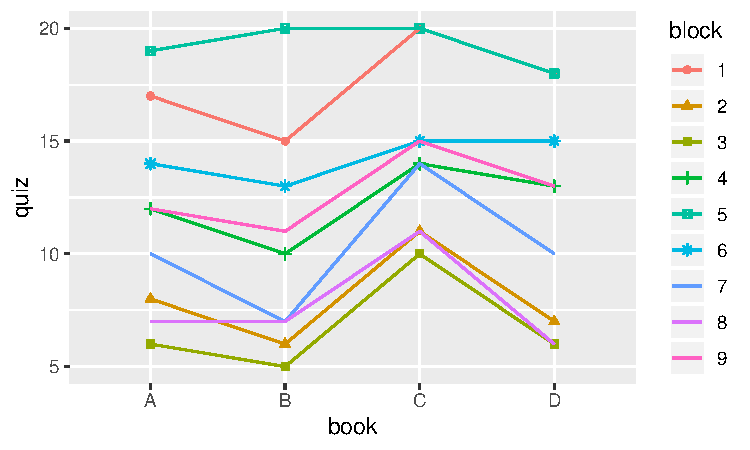
\includegraphics{Chapter-15-Assignment-R-Skeleton--2020spring_files/figure-latex/unnamed-chunk-21-1} \end{center}

\hypertarget{means-plot-1}{%
\subsubsection{Means Plot}\label{means-plot-1}}

\begin{center}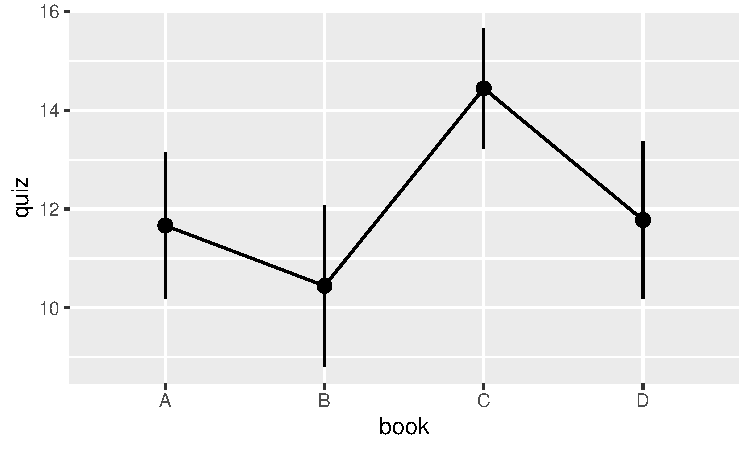
\includegraphics{Chapter-15-Assignment-R-Skeleton--2020spring_files/figure-latex/unnamed-chunk-22-1} \end{center}

\clearpage

\hypertarget{b-4a-rm-anova-display-all-sums-of-squares-components}{%
\subsubsection{15B-4a RM ANOVA: display all Sums-of-Squares
components}\label{b-4a-rm-anova-display-all-sums-of-squares-components}}

\textbf{TEXTBOOK QUESTION:} \emph{(a) Perform an RM ANOVA on the data,
and present the results of your ANOVA in a summary table. Does it make a
difference which textbook the professor uses? (b) Considering your
answer to part a, what type of error could you be making (Type I or Type
II)?}

\textbf{DIRECTIONS:} Perform a Repeated Measures ANOVA for quiz scores
under the four books to determine if the text has an effect. Make sure
to save your model (\texttt{fit\_textbook}), so that you can add
\texttt{\$aov} at the end of the name to extract all the
Sums-of-Squares.

\begin{Shaded}
\begin{Highlighting}[]
\CommentTok{# RM ANOVA: display all Sums-of-Squares components}
\end{Highlighting}
\end{Shaded}

\clearpage

\hypertarget{b-4c-rm-anova-gg-correction-for-lack-of-sericity}{%
\subsubsection{15B-4c RM ANOVA: GG correction for lack of
sericity}\label{b-4c-rm-anova-gg-correction-for-lack-of-sericity}}

\textbf{TEXTBOOK QUESTION:} \emph{(c) Would your F ratio from part a be
significant at the .01 level if you were to assume a maximum violation
of the sphericity assumption? Explain. }

\textbf{DIRECTIONS:} Run the name of the model \texttt{fit\_textbook}
alone to extract the adjusted degrees of freedom and F-test. The
sums-of-squares for the corrected test are the same as for the
uncorrected you just did.

\begin{Shaded}
\begin{Highlighting}[]
\CommentTok{# RM ANOVA: GG correction for lack of sphericity}
\end{Highlighting}
\end{Shaded}

\clearpage

\hypertarget{b-4d-rm-anova-post-hoc-with-tukeys-hsd-correction}{%
\subsubsection{15B-4d RM ANOVA: post-hoc with Tukey's HSD
correction}\label{b-4d-rm-anova-post-hoc-with-tukeys-hsd-correction}}

\textbf{TEXTBOOK QUESTION:} \emph{(d) Test all the pairs of means with
Tukey's HSD, using the error term from the RM ANOVA. Which pairs differ
significantly at the .05 level?}

\textbf{DIRECTIONS:} Conduct all possible post hoc pairwise tests on
\texttt{fit\_audience} using Tukey's HSD.

\begin{Shaded}
\begin{Highlighting}[]
\CommentTok{# RM ANOVA: post hoc all pairwise tests with Tukey's HSD correction}
\end{Highlighting}
\end{Shaded}

\begin{center}\rule{0.5\linewidth}{\linethickness}\end{center}

\textbf{Means Plot (model based)}

\textbf{DIRECTIONS:} Construct a means plot of \texttt{fit\_audience}
using \texttt{emmeans::emmip(\textasciitilde{}\ RM\_var)} to help
interpret the direction of any significant differences.

\clearpage

\hypertarget{b-5a-1-way-anova-treat-studnets-as-independent}{%
\subsubsection{15B-5a 1-Way ANOVA (treat studnets as
independent)}\label{b-5a-1-way-anova-treat-studnets-as-independent}}

\textbf{TEXTBOOK QUESTION:} \emph{(a) Perform a one-way
independent-groups ANOVA on the data from Exercise 4.}

\textbf{DIRECTIONS:} Perform the ANOVA with the \texttt{book} as an
between-subjects factor, instead of a within-subjects factor (ignoring
matching) for quiz scores to determine if the text has an effect. Make
sure to save your model (\texttt{fit\_book1way}), so that you can add
\texttt{\$aov} at the end of the name to extract all the
Sums-of-Squares.

\begin{Shaded}
\begin{Highlighting}[]
\CommentTok{# 1-way ANOVA: 1 between-subject factor}
\end{Highlighting}
\end{Shaded}

\begin{center}\rule{0.5\linewidth}{\linethickness}\end{center}

\textbf{TEXTBOOK QUESTION:} \emph{(b) Does choice of text make a
significant difference when the groups of subjects are considered to be
independent (i.e., the matching is ignored)? (c) Comparing your solution
to this exercise with your solution to Exercise 4, which part of the F
ratio remains unchanged? What can you say about the advantages of
matching in this case?}

\clearpage

\hypertarget{memory_wide---repeated-measures-design-stimulis-effect-on-memory-recall}{%
\subsection{\texorpdfstring{\texttt{memory\_wide} - Repeated Measures
Design: Stimuli's Effect on Memory
Recall}{memory\_wide - Repeated Measures Design: Stimuli's Effect on Memory Recall}}\label{memory_wide---repeated-measures-design-stimulis-effect-on-memory-recall}}

\textbf{TEXTBOOK QUESTION:} \emph{A neuropsychologist is exploring
short-term memory deficits in people who have suffered damage to the
left cerebral hemisphere. He suspects that memory for some types of
material will be more affected than memory for other types. To test this
hypothesis he presented six brain-damaged subjects with stimuli
consisting of strings of digits, strings of letters, and strings of
digits and letters mixed. The longest string that each subject in each
stimulus condition could repeat correctly is presented in the following
table. (One subject was run in each of the six possible orders.)}

\begin{verbatim}
  id digit letter mixed
1  1     6      5     6
2  2     8      7     5
3  3     7      7     4
4  4     8      5     8
5  5     6      4     7
6  6     7      6     5
\end{verbatim}

\hypertarget{restructure-from-wide-to-long-format-4}{%
\subsubsection{Restructure from wide to long
format}\label{restructure-from-wide-to-long-format-4}}

\begin{verbatim}
      id stimuli recall
1      1   digit      6
2      1  letter      5
3      1   mixed      6
4      2   digit      8
... <NA>    <NA>    ...
15     5   mixed      7
16     6   digit      7
17     6  letter      6
18     6   mixed      5
\end{verbatim}

\clearpage

\hypertarget{summary-statistics-2}{%
\subsubsection{Summary Statistics}\label{summary-statistics-2}}

\begin{longtable}[]{@{}llll@{}}
\toprule
& digit & letter & mixed\tabularnewline
\midrule
\endhead
& n = 6 & n = 6 & n = 6\tabularnewline
recall & & &\tabularnewline
& 7.0 (0.9) & 5.7 (1.2) & 5.8 (1.5)\tabularnewline
\bottomrule
\end{longtable}

\hypertarget{person-profile-plot-4}{%
\subsubsection{Person-Profile Plot}\label{person-profile-plot-4}}

\begin{center}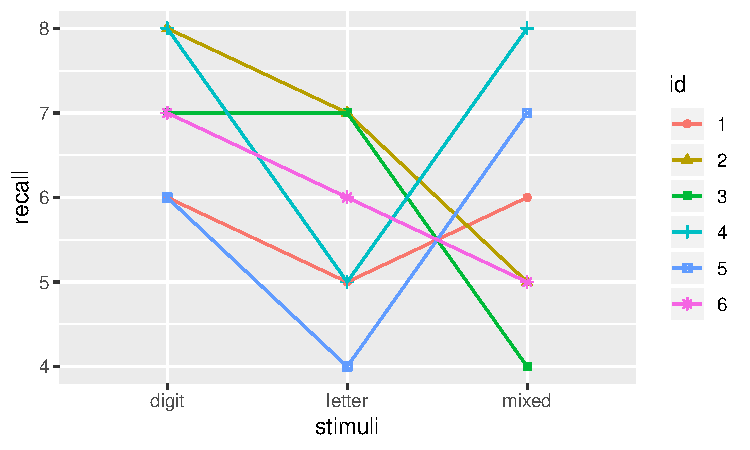
\includegraphics{Chapter-15-Assignment-R-Skeleton--2020spring_files/figure-latex/unnamed-chunk-32-1} \end{center}

\hypertarget{means-plot-2}{%
\subsubsection{Means Plot}\label{means-plot-2}}

\begin{center}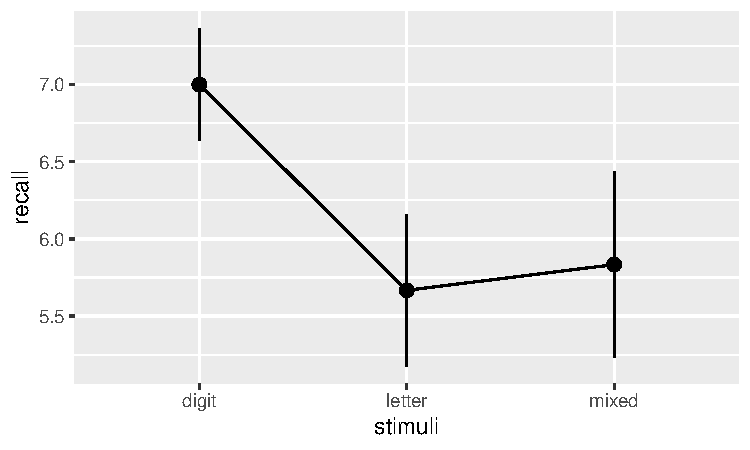
\includegraphics{Chapter-15-Assignment-R-Skeleton--2020spring_files/figure-latex/unnamed-chunk-33-1} \end{center}

\clearpage

\hypertarget{b-6a-rm-anova-with-sphericity-test-and-corrections}{%
\subsubsection{15B-6a RM ANOVA: with sphericity test and
corrections}\label{b-6a-rm-anova-with-sphericity-test-and-corrections}}

\textbf{TEXTBOOK QUESTION:} \emph{(a) Perform an RM ANOVA. Is your
calculated F value significant at the .05 level?}

\textbf{DIRECTIONS:} Perform a Repeated Measures ANOVA for recall under
the three stimuli to determine if the type of stimuli has an effect.
Save it as the name \texttt{fit\_memory} and then use the
\texttt{summary()} function display additional output.

\begin{Shaded}
\begin{Highlighting}[]
\CommentTok{# RM ANOVA: Mauchle Tests for Sphericity and Corrections applied}
\end{Highlighting}
\end{Shaded}

\clearpage

\hypertarget{b-6b-rm-anova-gg-corretion-for-lack-of-sphericity}{%
\subsubsection{15B-6b RM ANOVA: GG corretion for lack of
sphericity}\label{b-6b-rm-anova-gg-corretion-for-lack-of-sphericity}}

\textbf{TEXTBOOK QUESTION:} \emph{(b) Would your conclusion in part a
change if you could not assume that sphericity exists in the population
underlying this experiment? Explain. (c) Based on the graph you drew of
these data for Exercise 15A2, would you say that the RM ANOVA is
appropriate for these data? Explain.}

\textbf{DIRECTIONS:} Run the name of the model \texttt{fit\_memory}
alone to extract the adjusted degrees of freedom and F-test. The
sums-of-squares for the corrected test are the same as for the
uncorrected you just did.

\begin{Shaded}
\begin{Highlighting}[]
\CommentTok{# RM ANOVA: GG correction for lack of sphericity}
\end{Highlighting}
\end{Shaded}

\clearpage

\hypertarget{b-6d-rm-anova-post-hoc-with-fishers-lds-correction}{%
\subsubsection{15B-6d RM ANOVA: post-hoc with Fisher's LDS
correction}\label{b-6d-rm-anova-post-hoc-with-fishers-lds-correction}}

\textbf{TEXTBOOK QUESTION:} \emph{(d) Test all the possible pairs of
means with separate matched t tests (or two-group RM ANOVAs) at the .01
level.}

\textbf{DIRECTIONS:} Conduct all possible post hoc pairwise tests on
\texttt{fit\_memory} using Fisher's LSD.

\begin{Shaded}
\begin{Highlighting}[]
\CommentTok{# RM ANOVA: post hoc all pairwise tests with Fisher's LSD correction}
\end{Highlighting}
\end{Shaded}

\begin{center}\rule{0.5\linewidth}{\linethickness}\end{center}

\textbf{Means Plot (model based)}

\textbf{DIRECTIONS:} Construct a means plot of \texttt{fit\_audience}
using \texttt{emmeans::emmip(\textasciitilde{}\ RM\_var)} to help
interpret the direction of any significant differences.

\begin{Shaded}
\begin{Highlighting}[]
\CommentTok{# RM ANOVA: means plot}
\end{Highlighting}
\end{Shaded}

\clearpage

\hypertarget{section-c}{%
\section{SECTION C}\label{section-c}}

\hypertarget{import-data-define-factors-and-compute-new-variables}{%
\subsection{Import Data, Define Factors, and Compute New
Variables}\label{import-data-define-factors-and-compute-new-variables}}

Import Data, Define Factors, and Compute New Variables

\begin{itemize}
\tightlist
\item
  Make sure the \textbf{dataset} is saved in the same \emph{folder} as
  this file
\item
  Make sure the that \emph{folder} is the \textbf{working directory}
\end{itemize}

\begin{quote}
NOTE: I added the second line to convert all the variables names to
lower case. I still kept the \texttt{F} as a capital letter at the end
of the five factor variables.
\end{quote}

\begin{Shaded}
\begin{Highlighting}[]
\NormalTok{ihno_clean <-}\StringTok{ }\KeywordTok{read_excel}\NormalTok{(}\StringTok{"Ihno_dataset.xls"}\NormalTok{) }\OperatorTok\StringTok{ }
\StringTok{  }\NormalTok{dplyr}\OperatorTok{::}\KeywordTok{rename_all}\NormalTok{(tolower) }\OperatorTok\StringTok{ }
\StringTok{  }\NormalTok{dplyr}\OperatorTok{::}\KeywordTok{mutate}\NormalTok{(}\DataTypeTok{genderF =} \KeywordTok{factor}\NormalTok{(gender, }
                                 \DataTypeTok{levels =} \KeywordTok{c}\NormalTok{(}\DecValTok{1}\NormalTok{, }\DecValTok{2}\NormalTok{),}
                                 \DataTypeTok{labels =} \KeywordTok{c}\NormalTok{(}\StringTok{"Female"}\NormalTok{, }
                                            \StringTok{"Male"}\NormalTok{))) }\OperatorTok\StringTok{ }
\StringTok{  }\NormalTok{dplyr}\OperatorTok{::}\KeywordTok{mutate}\NormalTok{(}\DataTypeTok{majorF =} \KeywordTok{factor}\NormalTok{(major, }
                                \DataTypeTok{levels =} \KeywordTok{c}\NormalTok{(}\DecValTok{1}\NormalTok{, }\DecValTok{2}\NormalTok{, }\DecValTok{3}\NormalTok{, }\DecValTok{4}\NormalTok{,}\DecValTok{5}\NormalTok{),}
                                \DataTypeTok{labels =} \KeywordTok{c}\NormalTok{(}\StringTok{"Psychology"}\NormalTok{,}
                                           \StringTok{"Premed"}\NormalTok{,}
                                           \StringTok{"Biology"}\NormalTok{,}
                                           \StringTok{"Sociology"}\NormalTok{,}
                                           \StringTok{"Economics"}\NormalTok{))) }\OperatorTok\StringTok{ }
\StringTok{  }\NormalTok{dplyr}\OperatorTok{::}\KeywordTok{mutate}\NormalTok{(}\DataTypeTok{reasonF =} \KeywordTok{factor}\NormalTok{(reason,}
                                 \DataTypeTok{levels =} \KeywordTok{c}\NormalTok{(}\DecValTok{1}\NormalTok{, }\DecValTok{2}\NormalTok{, }\DecValTok{3}\NormalTok{),}
                                 \DataTypeTok{labels =} \KeywordTok{c}\NormalTok{(}\StringTok{"Program requirement"}\NormalTok{,}
                                            \StringTok{"Personal interest"}\NormalTok{,}
                                            \StringTok{"Advisor recommendation"}\NormalTok{))) }\OperatorTok\StringTok{ }
\StringTok{  }\NormalTok{dplyr}\OperatorTok{::}\KeywordTok{mutate}\NormalTok{(}\DataTypeTok{exp_condF =} \KeywordTok{factor}\NormalTok{(exp_cond,}
                                   \DataTypeTok{levels =} \KeywordTok{c}\NormalTok{(}\DecValTok{1}\NormalTok{, }\DecValTok{2}\NormalTok{, }\DecValTok{3}\NormalTok{, }\DecValTok{4}\NormalTok{),}
                                   \DataTypeTok{labels =} \KeywordTok{c}\NormalTok{(}\StringTok{"Easy"}\NormalTok{,}
                                              \StringTok{"Moderate"}\NormalTok{,}
                                              \StringTok{"Difficult"}\NormalTok{,}
                                              \StringTok{"Impossible"}\NormalTok{))) }\OperatorTok\StringTok{ }
\StringTok{  }\NormalTok{dplyr}\OperatorTok{::}\KeywordTok{mutate}\NormalTok{(}\DataTypeTok{coffeeF =} \KeywordTok{factor}\NormalTok{(coffee,}
                                 \DataTypeTok{levels =} \KeywordTok{c}\NormalTok{(}\DecValTok{0}\NormalTok{, }\DecValTok{1}\NormalTok{),}
                                 \DataTypeTok{labels =} \KeywordTok{c}\NormalTok{(}\StringTok{"Not a regular coffee drinker"}\NormalTok{,}
                                            \StringTok{"Regularly drinks coffee"}\NormalTok{)))  }\OperatorTok\StringTok{ }
\StringTok{  }\NormalTok{dplyr}\OperatorTok{::}\KeywordTok{mutate}\NormalTok{(}\DataTypeTok{hr_base_bps =}\NormalTok{ hr_base }\OperatorTok{/}\StringTok{ }\DecValTok{60}\NormalTok{) }
\end{Highlighting}
\end{Shaded}

\clearpage

\hypertarget{ihno_clean---repeated-measures-design-effect-of-time-expereiment-on-anxiety-levels-performed-independently-by-gender}{%
\subsection{\texorpdfstring{\texttt{ihno\_clean} - Repeated Measures
Design: Effect of Time (expereiment) on Anxiety levels (performed
INDEPENDENTLY by
GENDER)}{ihno\_clean - Repeated Measures Design: Effect of Time (expereiment) on Anxiety levels (performed INDEPENDENTLY by GENDER)}}\label{ihno_clean---repeated-measures-design-effect-of-time-expereiment-on-anxiety-levels-performed-independently-by-gender}}

\textbf{TEXTBOOK QUESTION:} \emph{(a) Use Split File to perform separate
RM ANOVAs for men and women to test for a significant change in anxiety
level over time (baseline, prequiz, and postquiz). Use Options to
request pairwise tests. Write up the results in APA style.}

\begin{Shaded}
\begin{Highlighting}[]
\NormalTok{ihno_clean }\OperatorTok\StringTok{ }
\StringTok{  }\NormalTok{dplyr}\OperatorTok{::}\KeywordTok{select}\NormalTok{(sub_num, anx_base, anx_pre, anx_post) }\OperatorTok\StringTok{ }
\StringTok{  }\KeywordTok{head}\NormalTok{(}\DataTypeTok{n =} \DecValTok{4}\NormalTok{)}
\end{Highlighting}
\end{Shaded}

\begin{verbatim}
# A tibble: 4 x 4
  sub_num anx_base anx_pre anx_post
    <dbl>    <dbl>   <dbl>    <dbl>
1       1       17      22       20
2       2       17      19       16
3       3       19      14       15
4       4       19      13       16
\end{verbatim}

\hypertarget{restructure-from-wide-to-long-format-5}{%
\subsubsection{Restructure from wide to long
format}\label{restructure-from-wide-to-long-format-5}}

\begin{Shaded}
\begin{Highlighting}[]
\CommentTok{#Restructure: wide-to-long}
\NormalTok{ihno_anx_long <-}\StringTok{ }\NormalTok{ihno_clean }\OperatorTok\StringTok{ }
\StringTok{  }\NormalTok{tidyr}\OperatorTok{::}\KeywordTok{pivot_longer}\NormalTok{(}\DataTypeTok{cols =} \KeywordTok{c}\NormalTok{(anx_base, anx_pre, anx_post),}
                      \DataTypeTok{names_to =} \StringTok{"time"}\NormalTok{,}
                      \DataTypeTok{names_ptypes =} \KeywordTok{list}\NormalTok{(}\DataTypeTok{time =} \KeywordTok{factor}\NormalTok{()),}
                      \DataTypeTok{names_prefix =} \StringTok{"anx_"}\NormalTok{,}
                      \DataTypeTok{values_to =} \StringTok{"anxiety"}\NormalTok{) }\OperatorTok\StringTok{ }
\StringTok{  }\NormalTok{dplyr}\OperatorTok{::}\KeywordTok{arrange}\NormalTok{(sub_num, time)}
\end{Highlighting}
\end{Shaded}

\begin{Shaded}
\begin{Highlighting}[]
\NormalTok{ihno_anx_long }\OperatorTok\StringTok{ }
\StringTok{  }\NormalTok{dplyr}\OperatorTok{::}\KeywordTok{select}\NormalTok{(sub_num, time, anxiety) }\OperatorTok\StringTok{ }
\StringTok{  }\KeywordTok{head}\NormalTok{(}\DataTypeTok{n =} \DecValTok{12}\NormalTok{)}
\end{Highlighting}
\end{Shaded}

\begin{verbatim}
# A tibble: 12 x 3
   sub_num time  anxiety
     <dbl> <fct>   <dbl>
 1       1 base       17
 2       1 pre        22
 3       1 post       20
 4       2 base       17
 5       2 pre        19
 6       2 post       16
 7       3 base       19
 8       3 pre        14
 9       3 post       15
10       4 base       19
11       4 pre        13
12       4 post       16
\end{verbatim}

\clearpage

\hypertarget{c-1a-rm-anova-twice-with-sphericity-test-and-corrections}{%
\subsubsection{15C-1a RM ANOVA (twice): with sphericity test and
corrections}\label{c-1a-rm-anova-twice-with-sphericity-test-and-corrections}}

\textbf{RESTRICT to just FEMALES}

\textbf{DIRECTIONS:} Perform a Repeated Measures ANOVA for anxiety at
all three time points to determine if the experiment had an effect. Make
sure to preceed the ANOVA with a \texttt{dplyr::filter()} step to
restrict to just \texttt{genderF\ ==\ "Female}. Save it as the name
\texttt{fit\_anx\_female} and then use the \texttt{summary()} function
display additional output.

\begin{Shaded}
\begin{Highlighting}[]
\CommentTok{# RM ANOVA: Mauchle Tests for Sphericity with and without corrections applied}
\end{Highlighting}
\end{Shaded}

\clearpage

\textbf{DIRECTIONS:} If, and only if, the omnibus F test yielded
evidence of at least one time point having a different average anxiety
FOR WOMEN, follow up with post hoc pairs tests based on the ANOVA model.

\begin{Shaded}
\begin{Highlighting}[]
\CommentTok{# RM ANOVA: post hoc all pairwise tests with Fisher's LSD correction}
\end{Highlighting}
\end{Shaded}

\begin{center}\rule{0.5\linewidth}{\linethickness}\end{center}

\textbf{Means Plot (model based)}

\textbf{DIRECTIONS:} If, and only if, the omnibus F test yielded
evidence of at least one time point having a different average anxiety
FOR WOMEN construct a means plot of \texttt{fit\_audience} using
\texttt{emmeans::emmip(\textasciitilde{}\ RM\_var)} to help interpret
the direction of any significant differences.

\begin{Shaded}
\begin{Highlighting}[]
\CommentTok{# Means Plot: model based}
\end{Highlighting}
\end{Shaded}

\clearpage

\textbf{RESTRICT to just MALES}

\textbf{DIRECTIONS:} Perform a Repeated Measures ANOVA for anxiety at
all three time points to determine if the experiment had an effect. Make
sure to preceed the ANOVA with a \texttt{dplyr::filter()} step to
restrict to just \texttt{genderF\ ==\ "Male}. Save it as the name
\texttt{fit\_anx\_male} and then use the \texttt{summary()} function
display additional output.

\begin{Shaded}
\begin{Highlighting}[]
\CommentTok{# RM ANOVA: Mauchle Tests for Sphericity with and without corrections applied}
\end{Highlighting}
\end{Shaded}

\clearpage

\textbf{DIRECTIONS:} If, and only if, the omnibus F test yielded
evidence of at least one time point having a different average anxiety
FOR MEN, follow up with post hoc pairs tests based on the ANOVA model.

\begin{Shaded}
\begin{Highlighting}[]
\CommentTok{# RM ANOVA: post hoc all pairwise tests with Fisher's LSD correction}
\end{Highlighting}
\end{Shaded}

\begin{center}\rule{0.5\linewidth}{\linethickness}\end{center}

\textbf{Means Plot (model based)}

\textbf{DIRECTIONS:} If, and only if, the omnibus F test yielded
evidence of at least one time point having a different average anxiety
FOR MEN, construct a means plot of \texttt{fit\_audience} using
\texttt{emmeans::emmip(\textasciitilde{}\ RM\_var)} to help interpret
the direction of any significant differences.

\begin{Shaded}
\begin{Highlighting}[]
\CommentTok{# Means Plot: model based}
\end{Highlighting}
\end{Shaded}

\clearpage

\hypertarget{c-1b-paired-t-tests-choose-2-at-a-time}{%
\subsubsection{15C-1b Paired t-Tests: choose 2 at a
time}\label{c-1b-paired-t-tests-choose-2-at-a-time}}

\textbf{TEXTBOOK QUESTION:} \emph{(b) Using ANALYZE/Compare Means ,
perform matched t tests for each pair of RM levels, and then compare
these p values to those produced in the Pairwise Comparisons results box
of the RM ANOVA.}

\textbf{DIRECTIONS:} If, and only if, the omnibus F test yielded
evidence of at least one time point having a different average anxiety
FOR WOMEN, follow up with post hoc pairs tests NOT based on the ANOVA
model. Instead, increase your \texttt{dplyr::filter()} to include
requiring only 2 of the 3 time points (eg.
\texttt{time\ \%in\%\ c("baseline",\ "pre-quiz")}). You will have to do
this 3 times, as there are three ways to choose a pair from three
options.

\begin{Shaded}
\begin{Highlighting}[]
\CommentTok{# Paired T-test: filter - women & baseline/pre-quiz}
\end{Highlighting}
\end{Shaded}

\begin{Shaded}
\begin{Highlighting}[]
\CommentTok{# Paired T-test: filter - women & baseline or post-quiz}
\end{Highlighting}
\end{Shaded}

\begin{Shaded}
\begin{Highlighting}[]
\CommentTok{# Paired T-test: filter - women & pre-quiz/post-quiz}
\end{Highlighting}
\end{Shaded}

\clearpage

\textbf{DIRECTIONS:} If, and only if, the omnibus F test yielded
evidence of at least one time point having a different average anxiety
FOR MEN, follow up with post hoc pairs tests NOT based on the ANOVA
model. Instead, increase your \texttt{dplyr::filter()} to include
requiring only 2 of the 3 time points (eg.
\texttt{time\ \%in\%\ c("baseline",\ "pre-quiz")}). You will have to do
this 3 times, as there are three ways to choose a pair from three
options.

\begin{Shaded}
\begin{Highlighting}[]
\CommentTok{# Paired T-test: filter - men & baseline/pre-quiz}
\end{Highlighting}
\end{Shaded}

\begin{Shaded}
\begin{Highlighting}[]
\CommentTok{# Paired T-test: filter - men & baseline or post-quiz}
\end{Highlighting}
\end{Shaded}

\begin{Shaded}
\begin{Highlighting}[]
\CommentTok{# Paired T-test: filter - men & pre-quiz/post-quiz}
\end{Highlighting}
\end{Shaded}

\clearpage

\hypertarget{ihno_clean---repeated-measures-design-effect-of-experiemnt-with-vs-without-the-experimental-item-on-stat-quiz}{%
\subsection{\texorpdfstring{\texttt{ihno\_clean} - Repeated Measures
Design: Effect of experiemnt (with vs without the experimental item) on
Stat
Quiz}{ihno\_clean - Repeated Measures Design: Effect of experiemnt (with vs without the experimental item) on Stat Quiz}}\label{ihno_clean---repeated-measures-design-effect-of-experiemnt-with-vs-without-the-experimental-item-on-stat-quiz}}

\textbf{TEXTBOOK QUESTION:} \emph{Perform an RM ANOVA to determine
whether there is a significant difference in mean scores between the
experimental stats quiz and the regular stats quiz. Compare this F ratio
with the matched t value you obtained from computer exercise \#3 in
Chapter 11.}

\begin{Shaded}
\begin{Highlighting}[]
\NormalTok{ihno_clean }\OperatorTok\StringTok{ }
\StringTok{  }\NormalTok{dplyr}\OperatorTok{::}\KeywordTok{select}\NormalTok{(sub_num, statquiz, exp_sqz) }\OperatorTok\StringTok{ }
\StringTok{  }\KeywordTok{head}\NormalTok{(}\DataTypeTok{n =} \DecValTok{5}\NormalTok{)}
\end{Highlighting}
\end{Shaded}

\begin{verbatim}
# A tibble: 5 x 3
  sub_num statquiz exp_sqz
    <dbl>    <dbl>   <dbl>
1       1        6       7
2       2        9      11
3       3        8       8
4       4        7       8
5       5        6       6
\end{verbatim}

\hypertarget{restructure-from-wide-to-long-format-6}{%
\subsubsection{Restructure from wide to long
format}\label{restructure-from-wide-to-long-format-6}}

\begin{Shaded}
\begin{Highlighting}[]
\NormalTok{ihno_statquiz_long <-}\StringTok{ }\NormalTok{ihno_clean }\OperatorTok\StringTok{ }
\StringTok{  }\NormalTok{tidyr}\OperatorTok{::}\KeywordTok{pivot_longer}\NormalTok{(}\DataTypeTok{cols =} \KeywordTok{c}\NormalTok{(statquiz, exp_sqz),}
                      \DataTypeTok{names_to =} \StringTok{"quiz_type"}\NormalTok{,}
                      \DataTypeTok{names_ptypes =} \KeywordTok{list}\NormalTok{(}\DataTypeTok{time =} \KeywordTok{factor}\NormalTok{()),}
                      \DataTypeTok{values_to =} \StringTok{"quiz_score"}\NormalTok{) }\OperatorTok\StringTok{ }
\StringTok{  }\NormalTok{dplyr}\OperatorTok{::}\KeywordTok{mutate}\NormalTok{(}\DataTypeTok{quiz_type =}\NormalTok{ quiz_type }\OperatorTok\StringTok{ }
\StringTok{                  }\NormalTok{forcats}\OperatorTok{::}\KeywordTok{fct_recode}\NormalTok{(}\StringTok{"Regular"}\NormalTok{ =}\StringTok{ "statquiz"}\NormalTok{,}
                                      \StringTok{"Experimental"}\NormalTok{ =}\StringTok{ "exp_sqz"}\NormalTok{))}
\end{Highlighting}
\end{Shaded}

\begin{Shaded}
\begin{Highlighting}[]
\NormalTok{ihno_statquiz_long }\OperatorTok\StringTok{ }
\StringTok{  }\NormalTok{dplyr}\OperatorTok{::}\KeywordTok{select}\NormalTok{(sub_num, quiz_type, quiz_score) }\OperatorTok\StringTok{ }
\StringTok{  }\KeywordTok{head}\NormalTok{(}\DataTypeTok{n =} \DecValTok{10}\NormalTok{)}
\end{Highlighting}
\end{Shaded}

\begin{verbatim}
# A tibble: 10 x 3
   sub_num quiz_type    quiz_score
     <dbl> <fct>             <dbl>
 1       1 Regular               6
 2       1 Experimental          7
 3       2 Regular               9
 4       2 Experimental         11
 5       3 Regular               8
 6       3 Experimental          8
 7       4 Regular               7
 8       4 Experimental          8
 9       5 Regular               6
10       5 Experimental          6
\end{verbatim}

\clearpage

\hypertarget{c-3-rm-anova-vs.-paired-t-test-only-2-groups}{%
\subsubsection{15C-3 RM ANOVA vs.~Paired t-test: only 2
groups}\label{c-3-rm-anova-vs.-paired-t-test-only-2-groups}}

\textbf{DIRECTIONS:} Perform a Repeated Measures ANOVA for recall under
the three stimuli to determine if the type of stimuli has an effect. Do
not save this model as a name; just run it without nameing/saving it.

\begin{quote}
NOTE: When the measure is only repeated twice, sphericity can not be
violated, so no such test are performed.
\end{quote}

\begin{Shaded}
\begin{Highlighting}[]
\CommentTok{# RM ANOVA: no correction for lack of sphericity }
\end{Highlighting}
\end{Shaded}

\begin{center}\rule{0.5\linewidth}{\linethickness}\end{center}

\textbf{DIRECTIONS:} Alternatively, since there are only two measures,
you can run this same analysis as a paired t.test, using
\texttt{t.test()}. Make sure you include \texttt{paired\ =\ TRUE}.

\begin{Shaded}
\begin{Highlighting}[]
\CommentTok{# Matched t-test: paired = TRUE}
\end{Highlighting}
\end{Shaded}

\end{document}
